%----------------------------------------------------------------------------
% Itt egy-egy alfejezetben nézném meg a BGP-hez és a vírus-/trendterjedéshez kapcsolódó policy-kat ill. egy harmadik alfejezetben néznék olyan extrákat, amiket nem tudok besorolni: ezek a tényleg elvontabbak. Tehát itt policy-kat sorolnék: BGP / vírus / extrák felosztásban. A 2.4 alfejezetben pedig írnék a szimulációról / a későbbi összehasonlításról, bár ezzel nagyon el vagyok csúszva (még semmit nem csináltam...)

%----------------------------------------------------------------------------
\chapter{A hálózatkutatás legfontosabb modelljei}\label{examples}
%----------------------------------------------------------------------------
\setcounter{note}{0}

Számos kutatás foglalkozik különböző hálózatokon terjedő információk vizsgálatával. Természetesen minden ilyen modellt le lehet írni az általánosított hálózati modellel, így a meghatározó policy-k azonosítása után vizsgálható \aref{modell}. fejezetben bemutatott, vagy azokhoz hasonló algebrákkal. Ebben a fejezetben bemutatom a hálózatkutatás leggyakrabban vizsgált modelljeit, és leírom a modellekhez tartozó meghatározó policy-ket is.\\

Az útvonalválasztás szempontjából alapvető különbség van a lokális- és a globális optimalizálás között. Míg globális optimalizálás esetén az egész hálózatot figyelembe véve választjuk meg a legjobb útvonalat, addig lokális optimalizálásnál csak a helyi viszonyok számítanak. Jelenleg a számítógépes hálózatokban a két legelterjedtebben használt policy kategória a ,,distance-vector''\footnote{Távolság-vektor módszerek, a Bellman-Ford algoritmusra épül.} és a ,,link-state''\footnote{Link-állapot módszerek, a Dijkstra algoritmusra épül.}. A módszerek abban különböznek, hogy a hálózatról milyen információkat gyűjtenek és hogyan, de abban megegyeznek, hogy globális optimumra törekszenek, tehát pl. a legrövidebb utat keresik meg. Ezzel szemben pl. a greedy routing\footnote{Mohó útvonalválasztás: A lokális helyzet optimumát választja.} csupán törekszik elérni globális optimumot, ám könnyen elakadhat, ha nem javítunk az alapalgoritmuson \cite{Routing_with_Guaranteed_Delivery_in_Adhoc_Wireless_Networks}. Könnyen belátható, hogy a vírusterjedés-jellegű feladatok lokális optimumra törekszenek, míg az Internetes útvonalválasztás globálisan optimalizál.

A másik szempont, ami meghatározó, az az, hogy a csomópontok felül tudják-e bírálni a csomagok terjedését abban az értelemben, hogy a küldő eredeti célját meg tudja-e valósítani akkor is, ha az útvonal mentén valamelyik csomópont ezt nem akarja. Feltehetjük-e, hogy a hibamentes csomagtovábbítás elsődleges prioritás minden hálózati csomópontnak (pl. kölcsönös bizalom megteremtése érdekében), vagy az egyes csomópontok viselkedhetnek önkényesen?

Mivel ezen két tulajdonság nem zárja ki egymást, a legtöbbször azzal az esettel állunk szemben, hogy nem tudunk egy problémát egyértelműen karakterizálni.


  %----------------------------------------------------------------------------
  \section{Vírusterjedés komplex hálózatokban}
  %----------------------------------------------------------------------------

  A vírusok terjedését és járvánnyá fejlődését sok évtizede vizsgálják. A járványok előrejelzése lehetőséget ad a tudósoknak, hogy megtervezzék a védőoltások ütemezését és az esetleges karanténok felállítását, ami jelentős hatással lehet egy adott betegség halálozási rátájára. A fertőző betegségek modellezése egy olyan eszköz, ami segítséget ad a fertőzés terjedésének vizsgálatához és a jövőbeli járványok elkerüléséhez stratégiákat lehet kidolgozni általa \cite{Epidemic_Modelling_An_Introduction}.

    %----------------------------------------------------------------------------
    \subsection{A vírusterjedés matematikai modellje}
    %----------------------------------------------------------------------------

    A legkorábbi ismert matematikai modell a fertőző betegségek terjedéséről Bernoullitól származik, aki a fekete himlőt vizsgálva megállapította, hogy ha mindenkit beoltanának a betegség ellen, akkor az átlagos életkor 26 év 7 hónapról 29 év 9 hónapra nőne \cite{Bernoulli_Blower}.

    Bernoulli munkája során természetesen még nem értette annyira a baktériumok és vírusok biológiáját, mint mi. A XX. század első felében Ronald Ross malária kutatásával kezdetét vette a modern elméleti fertőzés kutatás. Ezután nem sokkal, 1927-ben A. G. McKendrick and W. O. Kermack elismert munkája is megjelent, az ,,A Contribution to the Mathematical Theory of Epidemics''. Ez a determinisztikus modell sikeresen jelezte előre sok fertőző betegség viselkedését.\\

    Amikor nagy populációkat vizsgálunk, a determinisztikus modelleket használjuk, mert egy ilyenben a populáció egyedeit besorolhatjuk alcsoportokba, ami a fertőzés egy specifikus stádiumát jelenti. Ha a fertőzés átterjedése az egyik csoportról a másikra időben folytonos, a csoportok aktuális mérete matematikailag a deriválással fejezhető ki, így a modell leírható differenciál egyenletekkel. Ott játszik fontos szerepet a determinisztikusság, hogy egy ilyen modellben feltesszük, hogy egy csoport egyedszáma deriválható az idő szerint, ehhez viszont az kell, hogy a fertőződés kiszámíthatóan (nem véletlenszerűen) terjedjen tovább, más szóval a csoportok egyedszámának változása egyértelműen meghatározható az addigi múltból. Ezen modellek szakirodalmát és terminológiáját áttanulmányozva számos különböző mérőszámot és tulajdonságot találhatunk, de az alapmodell a következő három csoportot jelöli:
    \begin{itemize}
      \item \emph{S(t)}: A $t$ időpontig meg nem fertőzött egyedek száma, azaz akik még megfertőződhetnek.
      \item \emph{I(t)}: A $t$ időpontig megfertőzött egyedek száma, azaz akik tovább tudnak fertőzni.
      \item \emph{R(t)}: A $t$ időpontig megfertőzött, de mégsem I(t)-beli egyedek száma, azaz vagy meggyógyultak, vagy meghaltak. Ezen csoport egyedei már nem tudnak újra megbetegedni, sőt fertőzni sem fertőznek.
    \end{itemize}

    Egy egyed az $S(t) \rightarrow I(t) \rightarrow R(t)$ sorrendben halad a csoportok között. Egy fix méretű populációt feltételezve, $N~=~S+I+R$, a következő egyenleteket vezethetjük be \cite{Contributions_to_the_mathematical_theory_of_epidemics}:
    \begin{align}
      \frac{dS}{dt} &= - \beta S I\\
      \frac{dI}{dt} &= \beta S I - \gamma I\\
      \frac{dR}{dt} &= \gamma I
    \end{align}

    Ahol $\beta$ a kapcsolati ráta és $1/\gamma$ az átlagos fertőző periódus.

    Néhány feltételezést tettünk az egyenletek felírásához: (1) minden egyedet ugyanakkora valószínűséggel fertőz meg egy $\beta$ kapcsolati rátájú betegség, így minden fertőzött egyed $\beta N$ egészséges egyedet fertőz meg egy időegység alatt, illetve az egyedeknek átlagosan $S/N$ megfertőzhető kapcsolata van. Tehát a fertőzési ráta: az új betegek száma $\beta N (S/N)$, azaz amennyivel változik (nyilván csökken) $S$: $\beta N (S/N)I~=~\beta SI$.

    Ezután érthető a második és harmadik egyenlet: a fertőzöttek száma annyival nő, ahánnyal kevesebb egészséges lesz, illetve annyival fogy, ahány meghal vagy meggyógyul. A $\gamma$ jelöli az átlagos halálozási / felépülési rátát.

    Végül feltesszük, hogy a megfertőződés és a felépülés időben jóval gyorsabb folyamat, mint a születés és halálozás, így ezeket a faktorokat kihagyhatjuk a modellből.

    \begin{note}
      Természetesen számos következő szempontot figyelembe lehet még venni a modell mélyítése érdekében, ilyen például az előbb említett születés és halálozás; az $R \rightarrow S$ átmenet, azaz a fertőzésből való meggyógyulás után újra meg lehet betegedni; figyelembe lehet venni az úgynevezett lappangási időszakot, bevezetve egy újabb csoportot ($S \rightarrow \epsilon \rightarrow I \rightarrow R$); vagy a veleszületett betegséget is, azaz a fertőzött anyától elkapott betegséget is.\newline
      Jelen dolgozat szempontjából az alap SIR modell megfelelő.
    \end{note}

    %----------------------------------------------------------------------------
    \subsection{Vírusterjedés, mint útvonalválasztási probléma}
    %----------------------------------------------------------------------------

    A fertőző betegségek terjedése nem látszik útvonalválasztási kérdésnek sőt, semmilyen policy-t nem veszünk észre első ránézésre, ezért talán némi magyarázatot igényel a problémakör vizsgálata. A diplomadolgozat végső célja rejtett szabályok felismerése előre definiált policy primitívek segítségével tetszőleges hálózatban, így világos, hogy a vírusterjedést sem zárhatom ki a vizsgálatból.\\

    A fejezet bevezetőjében említett két tulajdonság közül az optimalizálás az, ami itt a legszembetűnőbb. Ha ugyanis nem úgy tekintünk a problémára, mint egy kétszereplős ,,háborúra'' (ember a vírus ellen), hanem úgy, mint a kis organizmusok egyéni útvonalválasztására, akkor látható, hogy lokális optimalizálásról van szó, hiszen minden egyes fertőző elem szeretne minél tovább élni újabb és újabb gazdatestet találva magának. Lévén itt nem a tipikus több lépésen keresztüli pont-pont routing-ról van szó, globális optimalizálási feladat legfeljebb az lehet, hogy minél több csomópont legyen fertőzött. Minden csomópontból arra fertőz tovább a vírus, amerre a legtöbb eséllyel fog továbbélni -- ez nyilván függ az adott vírus-egyedtől is -, azaz például a leggyengébb immunrendszerű ember felé. Ez alapján két policy-t mutatok be:

    \begin{itemize}
      \item Fertőzési-határ: A vírus-egyed legjobb továbbfertőzési policy-ja.
      \item Unió-fedés: A globális fertőzés policy-ja.
    \end{itemize}

      %----------------------------------------------------------------------------
      \subsubsection{Fertőzési-határ}
      %----------------------------------------------------------------------------

      A Fertőzési-határ policy alapú útvonalválasztás garantálja a legjobb túlélési esélyt egy vírus-egyed számára. Ennek a policy-nak az algebrája az $\mathcal{F}$ ($(0,1],~0,~max,~\geq$). Ennél az algebránál az élek súlya (egy (0,1] intervallumbeli valós szám) azt adja meg, hogy azt a csomópontot, ahová vezet, milyen valószínűséggel tudjuk megfertőzni, így nyilván a nagyobb jobb, a 0 pedig azt jelenti, hogy a csomópont $R(t)$-beli, azaz már biztosan nem lehet megfertőzni. Mivel az útvonalválasztás lokálisan optimalizál, ezért két alternatív élet a $\geq$ operátorral tudunk összehasonlítani, illetve a két él összeillesztésére a két él súlyának maximumát vesszük.

      %----------------------------------------------------------------------------
      \subsubsection{Unió-fedés}
      %----------------------------------------------------------------------------

      Az Unió-fedés policy szerinti útvonalválasztás célja, hogy lehetőleg olyan élen menjünk és fertőzzünk tovább, amit még nem használtak. Ennek a policy-nak a számítógépes vírusok tárgyalásánál van nagyobb szerepe, semmint a biológiai fertőzéseknél, hiszen ez alapján -- akár már fertőzött gépet is -- minden olyan élet saját felügyelet alá vehetünk, amit még nem találtunk meg, így például ügyelhetünk arra, hogy semelyik fertőzött gép ne tudja frissíteni a vírusirtójának a vírusdefiníciós adatbázisát.

      Az Unió-fedés policy algebrája az $\mathcal{U}$ ($\mathbb{N},~\infty,~f,~\leq$). Itt az élsúly egy természetes szám lehet és azt fejezi ki, hogy hányszor használták már fel egy útvonalválasztásban. Mivel a cél az, hogy minél ritkábban (optimálisan soha nem) használt utakat használjunk, a $\infty$ jelenti az átjárhatatlanságot és a $\leq$ az összehasonlító operátor. A több élből álló út súlyát az $f$ összegző függvény adja:
      $$f(e_1,e_2)~=~
      \begin{cases}
        e_1+e_2 & \text{ha } e_1*e_2 \neq 0 \\
        0 & \text{különben}
      \end{cases}$$
      Ezzel garantáljuk, hogy olyan esetben, amikor úgyis mindegy -- azaz nincs még fel nem használt él -- akkor az élek súlyának összegét vesszük, de amikor van olyan él, amit még nem használtunk, akkor azt biztosan fogjuk használni (hacsak nincs egy másik alternatív 0 súlyú út), hiszen a két élű út súlya 0 lesz.\newpage

  %----------------------------------------------------------------------------
  \section{Trendterjedés közösségi hálózatokban}
  %----------------------------------------------------------------------------

  A közösségi hálózatok az elmúlt 10 év egyik legmeghatározóbb jelensége, új korszakot nyitott az emberi kapcsolatokban. A kapcsolatháló elemzés a szociometriából indult, de annál bonyolultabb, időben is változó, nagyobb közösségek vizsgálatára alkalmas módszertan. A kapcsolatháló elemzési módszerek alkalmasak egy nagyobb csoport klikkjeinek és alcsoportjainak felrajzolására és megjelenítésére is. A kapcsolathálózati megközelítés kevésbé hangsúlyozza az egyéni cselekvés szerepét a struktúrák létrehozásában, nem az egyéni szándékból, hanem a struktúrák belső feszültségeiből jön létre a cselekvés mozgástere. A struktúra -- pl. egy elterjed trend -- e szemléletmód számára nem egy közvetlenül megmutatkozó adottság, hanem sokkal inkább a kapcsolatok hálójából bonyolultan kibontható szerveződés.

  A hálózati megközelítés előnye, hogy az adott hálózati struktúrákat, közösségeken belül kialakuló attribútumokat dinamikus módon, a változásokon keresztül is képes vizsgálni: a kapcsolatok és a környezet folytonosan változó mozgása mentén. A hálózat elemzéssel komplex módon tudjuk leírni vizsgált közösségi hálózatok működését \cite{Csaba_Pal}.\\

  A trend- vagy divatterjedés egy szociális hálóban lehetséges, ahol az egyik csomóponttal szimbolizált egyén felvesz egy szokást, elkezd hordani egy bizonyos ruhadarabot (vagy márkát), vagy bármi olyat tesz, amit ,,az átlag'' nem. Ha az ismerősei -- a kapcsolati hálóban szomszédos csomópontok -- észreveszik ezt az újdonságot és megtetszik nekik is, átveszik a forrástól. A problémakör alapvető kérdése, hogy mi határozza meg, hogy elterjed-e egy trend és divattá válik-e az egész hálózatban, vagy sem. Malcolm T. Gladwell brit-kanadai újságíró, író 2000-ben megjelent könyvében \cite{The_Tipping_Point} számos példát olvashatunk, hogy egyes szituációkban mikor érkezett el a fordulópont, mikor vált általános divattá valami. Ilyen példa a Hush Puppy cipőgyártó cég, mely egyik pillanatról a másikra a csőd széléről világszerte ismert márkává vált. Gladwell azt állítja, hogy a kulcs az úgynevezett \emph{Összekötőkön} múlik. Egy összekötő tipikusan hatalmas társasági kapcsolatrendszerrel rendelkezik, mely kapcsolatok többnyire gyenge kötelék csupán, emellett több mikrovilágba és szubkultúrába bejáratos. Az ilyen összekötőket kell megnyernie egy terméknek és ennek szinte automatikus következménye, hogy elterjed a termék és divattá válik. Duncan Watts ausztrál fizikus-matematikus-szociológus megkérdőjelezte Gladwell állítását, szerinte ugyanis nem az a meghatározó, hogy egy divat az összekötőktől indul-e, hanem az, hogy a közösség (akár az egész társadalom, akár csak egy szűkebb baráti kör) készen áll-e az adott divat elterjedésére. Tehát nem a forrás számít és annak befolyása, hanem az, hogy általánosságban a közösség egésze akarja-e a terméket.\\

    %----------------------------------------------------------------------------
    \subsection{Trendterjedés, mint útvonalválasztási probléma}
    %----------------------------------------------------------------------------

    A trendterjedés nagyon hasonlít a vírusterjedésre, hiszen maga a két eredeti modell is szinte egy az egyben megfeleltethető egymásnak. Természetesen a vírusterjedés esetén említett kiegészítéseket nem lehet egy az egyben átültetni és a trendterjedés terminológiájával leírni, de az alapmodell három csoportját ($S$, $I$, $R$) itt is azonosíthatjuk. Világos, hogy az optimalizálás lokalizáltsága erre a modellre is jellemző, hiszen nincs olyan divat, ami egy bizonyos emberre akar csak hatni, sokkal inkább mindenkire. Így ennek a problémakörnek is jellemző policy-ja lehet az \emph{Unió-fedés}.

    Útvonalválasztási szempontból a lényeges különbség, hogy a trendterjedésnél a csomópontoknak van döntő szerepe, nem az éleknek, azaz itt nem közös érdek, hogy egy divat elterjedjen (vagy akar az, hogy ne terjedjen el). Bárki mondhatja azt, hogy neki kifejezetten nem tetszik az elterjedő divat, ezért pl. lebeszéli az ismerőseit róla, vagy csak egyszerűen nem veszi át, így megállítja a terjedést, legalábbis a közvetlen közelében. Nyilvánvaló, hogy -- bár az elterjedés kulcsa az, hogy a társadalom készen áll-e -- egy \emph{Összekötő} nagyban hozzájárulhat a sikeres terjesztéshez, így preferálhatjuk ezen központi csomópontokat. Emellett az is szempont lehet, hogy nem a csomópontok befolyását vesszük alapul, hanem pusztán a mennyiségüket és egy adott útvonalválasztáskor minél hosszabb útra törekszünk. Egy másik alkalmazható heurisztika, hogy ha két csomópont közötti élen sok divat terjedt át, akkor ezt az élet érdemes felhasználni, illetve megfordítva, ha egy élen eddig kevés divat terjedt át, akkor valószínűleg nem olyan a két végpont kapcsolata, amin a divatok átterjedhetnek, így érdemes elkerülni az ilyen éleket. Ezek alapján a következő policy-kat definiálom:

    \begin{itemize}
      \item Összekötő-keresés: A nagy súlyú csomópontok felé irányító policy.
      \item Korai-elfogadó-keresés: A mindent átvevő csomópontok felé irányító policy.
    \end{itemize}

      %----------------------------------------------------------------------------
      \subsubsection{Összekötő-keresés}\label{osszekoto_kereses}
      %----------------------------------------------------------------------------

      Ez a policy azon csomópontokat részesíti előnyben, amelyeket a legbefolyásosabbnak ítélünk. A vírus- és trendterjedés hasonlóságából adódóan itt is lokális optimalizálásról beszélhetünk, így mindig azt a szomszédot fogjuk választani, aminek a legnagyobb a fokszáma. Az Összekötő-keresés algebrája a $\mathcal{O}$ ($(1,d),~0,~max,~\geq$). Az élek súlya:
      $\forall u,v \in V:~w(u,v)~=~max(deg(u),deg(v))$, tehát az összekötött csomópontok fokszámai közül a nagyobb és nyilván a több jobb. Az átjárhatatlanságot a 0 súly jelzi, míg több él súlyát a maximumuk határozza meg.

      %----------------------------------------------------------------------------
      \subsubsection{Korai-elfogadó-keresés}\label{korai_elfogado_kereses}
      %----------------------------------------------------------------------------

      A Korai-elfogadó-keresés policy azon éleket részesíti előnyben, melyeken az eddigi tapasztalat alapján sok divat átterjedt már. Ennek lényege nyilván az, hogy egy ilyen él olyan személyek közötti kapcsolatot jelöl, akik pl. megbíznak a másik ítéletében, vagy az egyikük felnéz a másikra, így átvesz tőle viselkedési formákat. A policy algebrája a $\mathcal{K}$ ($\mathbb{N},~-1,~+,~\geq$). Az élek súlya azt jelzi, hogy eddig mennyi divat terjedt át rajta, így a több a jobb, és nyilván a -1 súlyú élen nem tudunk átmenni. Több él összeillesztését az élsúlyok összegével súlyozunk.\newpage


  %----------------------------------------------------------------------------
  \section{Útvonalválasztás az Interneten}
  %----------------------------------------------------------------------------

  A útvonalválasztás kutatói rendszerint informatikai-, vagy számításelméleti szakemberek, ezért a kutatási célok legnagyobb része számítógépes hálózatok útvonalválasztásának vizsgálata, javítása. Ezen a területen általában az Internet gerinchálózatát szokták vizsgálni, hiszen ott jelentkeznek azok a skálázhatósági- és menedzsmentproblémák, amik az Internet 1970-es évekbeli tervezéséből származnak és ami miatt azt mondhatjuk, hogy az Internet hibáinak toldozása-foldozása már nem elég és alapvetően új megoldások szükségesek.\\

  Két alapvetően eltérő koncepció létezik a számítógépes hálózatok útvonalválasztásában, a tapasztalatok alapján előre becsült forgalmi viszonyoknak megfelelő centralizált kialakítás; illetve az aktuális forgalmi helyzet állandó figyelése alapján, az annak legjobban megfelelő irányítás. Legtöbbször az utóbbit valósítják meg, méghozzá elosztott változatban. Az Internet tervezése során több olyan szempontot is figyelembe vettek, melyeket az előző két alfejezetben nem tudunk tárgyalni. Ilyen például a routerekben lévő útvonaltáblák minél kisebb mérete (kisebb tár, olcsóbb és gyorsabban működő csomópont, illetve kisebb routingforgalom), emellett fontos szempont a routingforgalom minimalizálása, a robusztusság (hibás tábla esélyének minimalizálása: ,,fekete lyuk'', hurok, oszcilláció elkerülése) és végül az optimális útvonalak kijelölése (természetesen az út optimalitása az igénytől függ). Az egyik legfontosabb igény az elosztott működés, a decentralizáltság volt azért, hogy az útvonalválasztást a csomópontok végezzék.\\

  Ahogy fejlődött a világ, újabb feladatok és problémák jelentek meg, amelyet a szakemberek a hálózat tervezésekor még nem láttak előre. Olyan új technológiák jelentek meg, mint a mobiltelefonok és a hordozható számítógépek és velük együtt az igény a mobil routingra, azaz arra, hogy ne csak a számítógép, de az internet hozzáférés is legyen hordozható. Problémát jelent a multicast routing is, amikor egy adott csomagot több címzetthez szeretnénk eljuttatni. Ezen problémák hatékony megoldása kritikus feladat, alapvetően új megoldásokat kívánnak.

  Emellett pusztán a hálózat mérete is feszegeti az Internet teljesítőképességének jelenlegi határait. Mára az Internet óriásira nőtt és a 1990-es évek vége óta a mindennapi élet meghatározó részévé vált. 2000 és 2009 között 394 millióról 1,84 milliárd nőtt az Internet kapcsolattal rendelkezők száma\footnote{Market Information and Statistics, International Telecommunications Union, \url{http://www.itu.int/ITU-D/ict/statistics/}}. Ma már több, mint 2,4 milliárd\footnote{2.405.518.376 -- 2012. második negyedév, \url{http://www.internetworldstats.com/stats.htm} 2014. 05. 09} felhasználója van az Internetnek, és 2010-ben 12,5 milliárd Internetre csatlakoztatott eszköz volt. Ez azt jelenti, hogy minden élő emberre jutott 1,84 készülék. 2020-ra az Internetre kapcsolt eszközök száma elérheti az 50 milliárdot \cite{The_Internet_of_Things}.\newpage

  Útvonalválasztási szempontból az Internet routing egy klasszikus feladat, amikor a legszélesebb-, legrövidebb- és legmegbízhatóbb utakat keressük. Ezen policy-k algebráit már bemutattam, megtalálhatók a \aref{tab:table_algebrapeldak} táblázatban.

  \begin{figure}[!ht]
    \centering
    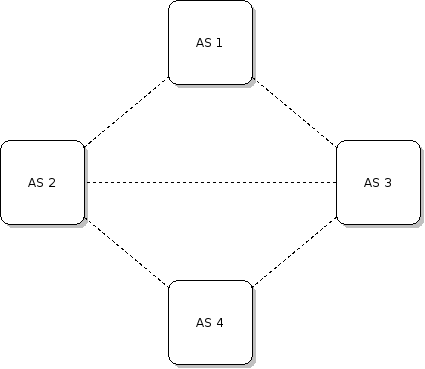
\includegraphics[width=70mm,keepaspectratio=true]{./figures/BGP_iranyitatlan.png}\hspace{5mm}
    % BGP_iranyitatlan.png: 425x369 pixel, 72dpi, 14.99x13.02 cm, bb=0 0 425 369
    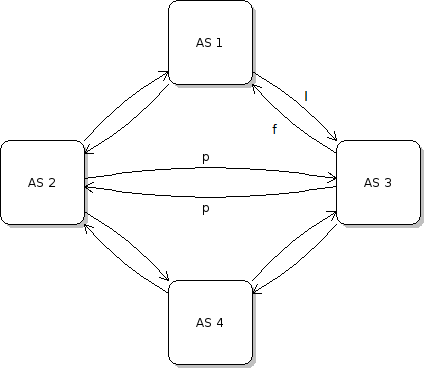
\includegraphics[width=70mm,keepaspectratio=true]{./figures/BGP_iranyitott_labeled.png}
    % BGP_iranyitott_labeled.png: 425x369 pixel, 72dpi, 14.99x13.02 cm, bb=0 0 425 369

    \caption{A BGP egyszerűsített képe és a völgymentesség szerinti irányítás.}
    \label{fig:figure_BGP}
  \end{figure}

  Érdemes megvizsgálni a BGP szabályrendszerét: a BGP routing policy-ja többszintű. A legalsó szint, a legalapvetőbb policy a völgymentesség. Ez azt jelenti, hogy az útvonalválasztásnál elsődleges szempont, hogy semelyik AS-nek ne kelljen fizetni olyan forgalomért, ami csak áthalad rajta. Ha a hierarchiában lefelé mutató éleket $l$-lel, a felfelé mutató éleket $f$-fel, a peering kapcsolatokat pedig $p$-vel jelöljük, akkor minden routing során kijelölt útvonal csak a következő alakban írható le: néhány (akár nulla) $f$ él, aztán maximum egy $p$ él, utána pedig néhány (akár nulla) $l$ él.\\

  Emellett, ha felhasználjuk a gráfbeágyazás és kompakt routing eredményeit, akkor egy új távolságfüggvénnyel és a csomópontok koordinátázásával megvalósítható az Internet tartományszintű gráfjában is egy elakadásmentes mohó útvonalválasztás \cite{DobreiBScSzakdolgozat}.

  \begin{figure}[h]
    \centering
    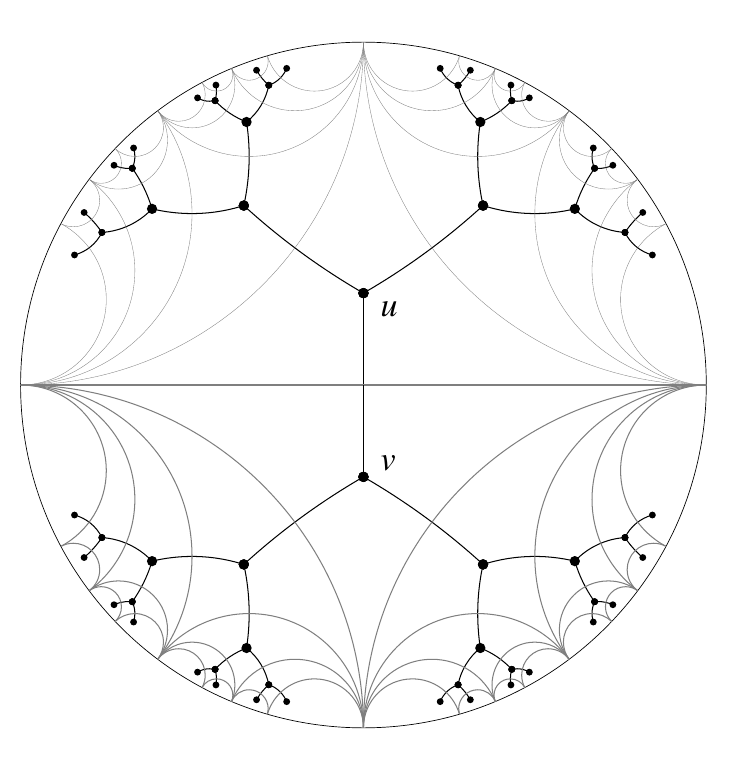
\includegraphics[width=70mm]{./figures/3-reg_disk.png}\hspace{5mm}
    % 3-reg_disk.png: 749x757 pixel, 96dpi, 19.81x20.03 cm, bb=0 0 562 568
    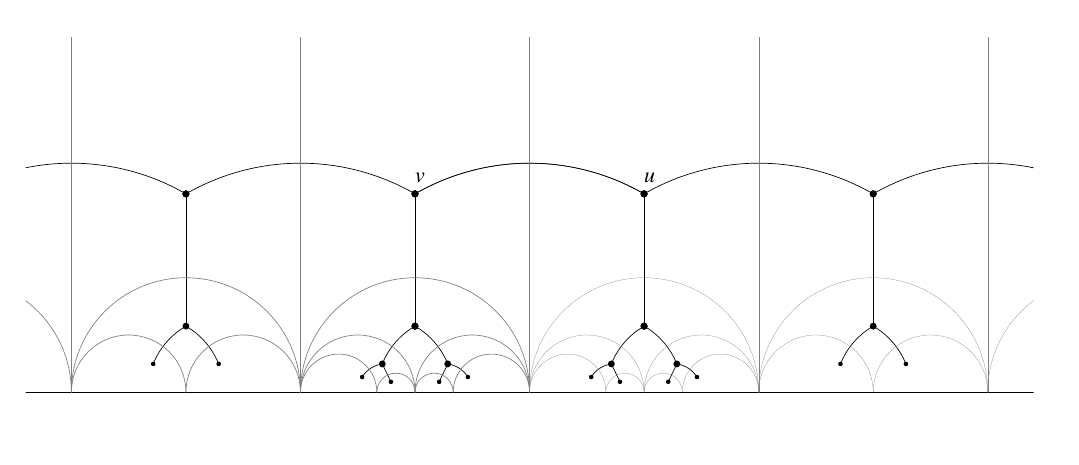
\includegraphics[width=70mm,keepaspectratio=true]{./figures/3-reg_half_plane.png}
    % 3-reg_half_plane.png: 1079x465 pixel, 96dpi, 28.54x12.30 cm, bb=0 0 809 349

    \caption{A hiperbolikus sík Poincaré-féle diszk modellje és a felső félsík modellje \cite{Klein07}.}
    \label{fig:figure_hiperbolikusabrak}
  \end{figure}

  A $\mathbb{H}$ hiperbolikus síknak többféle szemléltető modellje is van, ám a két legelterjedtebb a felső félsík modell és a Poincaré diszk modell, amiket \aref{fig:figure_hiperbolikusabrak} ábrán láthatunk is. A Poincaré modellben $\mathbb{H}$-t egy egységkörrel reprezentálják: $x^2~+~y^2~<~1$, a következő metrikával:
  \begin{align}
    ds^2~=~\frac{4(dx^2~+~dy^2)}{(1~-~x^2~-~y^2)^2}.
  \end{align}

  A felső félsík modellben $\mathbb{H}$-t a $\{\langle x,y\rangle ~|~y~>~0\}$ ponthalmaz írja le, ahol a metrika:

  \begin{align}
    ds^2~=~\frac{dx^2~+~dy^2}{y^2}.
  \end{align}

  Mindkét esetben a $\mathbb{H}$ pontjait komplex számokként kezeljük: $(x,y)~\in~\mathbb{R}^2:~z~=~x~+~yi$.

  Ezek alapján két új policy-t mutatok be:

  \begin{itemize}
    \item Hiperbolikus-távolság: Az elakadásmentes mohó útvonalválasztás policy-ja.
    \item Völgymentesség: A BGP alapvető, elsődleges policy-ja.
  \end{itemize}

      %----------------------------------------------------------------------------
      \subsubsection{Hiperbolikus-távolság}
      %----------------------------------------------------------------------------

      A hiperbolikus síkra ágyazott Internet gráf minden pontja egy $(x,y)$ koordinátapárral leírható. A policy algebrája a $\mathcal{H}$ ($\mathbb{R}^{+},~\infty,~f_{\mathbb{H}},~\leq$), ahol $f_{\mathbb{H}}$ egy viszonylag bonyolult függvény, definiálásához szükséges lenne több, itt nem részletezett ismeret a hiperbolikus geometria témaköréből (bővebben ld. \cite{Thurston97} 2. fejezetét).

      %----------------------------------------------------------------------------
      \subsubsection{Völgymentesség}
      %----------------------------------------------------------------------------

      A völgymentesség policy-nak az algebrája a $\mathcal{V}$ ($\{f,~l,~p\},\phi,\bigoplus_{\mathcal{V}},\preceq$),  ahol a $\bigoplus_{\mathcal{V}}$ \aref{tab:szumma_tab} táblázat szerinti\footnote{ Egy adott súlyú (típusú) úthoz hozzá akarnánk venni egy élet, akkor az út milyen súlyúvá (típusúvá) válna.}. Az előbbi szabály másik megfogalmazásban azt jelenti, hogy sem $l$-t, sem $p$-t nem követhet sem $p$, sem $f$.

      \begin{table}[ht]
        \footnotesize
        \centering
        \caption{A $\bigoplus_{\mathcal{V}}$ \cite{Compact_Policy_Routing}.}
        \begin{tabular}{ c | c c c }
          $\bigoplus$ & $f$ & $l$ & $p$\\
          \hline
          $f$ & $f$ & $l$ & $p$\\
          $l$ & $\phi$ & $l$ & $\phi$\\
          $p$ & $\phi$ & $p$ & $\phi$\\
        \end{tabular}\label{tab:szumma_tab}
      \end{table}\newpage

  %----------------------------------------------------------------------------
  \section{Egyéb algebrák}
  %----------------------------------------------------------------------------

  A minél részletesebb vizsgálat érdekében definiálok olyan policy-kat is, melyek vagy minden eddigi modellben használható lenne, vagy egyikben sem, így eddig nem volt lehetőségem bemutatni.

  A fejezet legelején felvázolt két dimenzió (optimalizálás, érdekek) mellett a harmadik karakterizálási lehetőség az időbeli lefolyás. Ha egy útvonalválasztási probléma tárgyalása során figyelembe vesszük az időt is, mint befolyásoló tényezőt, egy olyan új dimenziót ragadunk meg, mely minden modell routing-ját képes befolyásolni: ez az \emph{Időfüggés} policy. A vírus-terjedésnél elég csak arra gondolni, hogy télen könnyebben tud terjedni a fertőzés, és hasonlóan nyáron nagyobb valószínűséggel terjed egy fürdőruhadivat. Fontos azonban, hogy ez csak egy mellékes faktor, azaz egy alap policy mellett van értelme figyelembe venni az időpontot is. Az Internetes útvonalválasztás során időfüggést tapasztalhatunk, ha pl. egy terheléselosztó rendszer egy adott kérést másodpercenként váltakozva egyszer kiszolgál, egyszer pedig újrapróbálkozásra szólít fel.\\

  Másik érdekes policy, a trendterjedésnél említett leghosszabb út policy. Ennek olyan esetben van értelme, amikor nem a célba érkezés a legfontosabb, hanem maga az út. A vírus- és trendterjedésnél ez azért volt lényeges, hogy minél több embert elérjünk, de pl. a hangyák is így építik ki a bolyban az utakat, hogy egy esetleges betolakodó minél nagyobb valószínűséggel eltévedjen.

      %----------------------------------------------------------------------------
      \subsubsection{Leghosszabb-út}
      %----------------------------------------------------------------------------

      A leghosszabb-út policy adja az elérhető leghosszabb utat. Ebben az esetben az $\mathcal{L}$ algebra az $(1, 0,~+,~\geq)$ négyes. Ebben a policy-ban minden él konstans 1 súlyú, egy út súlya éppen az élszáma.

      %----------------------------------------------------------------------------
      \subsubsection{Időfüggés}
      %----------------------------------------------------------------------------
      Az Időfüggés policy lényege, hogy az időpontot\footnote{A lépték mértéke problémafüggő: lehet naponkénti éves periódusokkal, lehet } figyelembe véve néha átjárhatatlan egy-egy él. Ehhez szükséges egy alap policy is, amelyet ez ki tud egészíteni: $\mathcal{A}$. Jelölje $T_{e_i}$ az időpontok egy olyan halmazát, melyben $\mathcal{I}$ nem enged át forgalmat az $e_i$ élen. (A $T_{e_i}$ lehet akár egy $[t_0, \infty)$ intervallum is.) Így az $\mathcal{I}$ algebra: $(W_{\mathcal{A}},~\phi_{\mathcal{A}},~f,~\preceq_{\mathcal{A}})$, ahol
      $$f(e_1,e_2,t)~=~
      \begin{cases}
        \phi_{\mathcal{A}} & \text{ha } t \in T_{e_1} \cup T_{e_2}\\
        e_1 \bigoplus_{\mathcal{A}} e_2 & \text{különben}
      \end{cases}$$

      Azaz, alkalmas időpontban teljes egészében az $\mathcal{A}$ policy érvényesül, azonban minden élen bizonyos időpontokban nem lehet átmenni.\\

  %----------------------------------------------------------------------------
  \section{Összefoglaló}
  %----------------------------------------------------------------------------
  Ebben a fejezetben megvizsgáltam a hálózatkutatás szempontjából alapvető modelleket, melyeket a lokális- vagy globális optimalizálás és a közös- vagy egyéni érdekek követése tulajdonságok alapján karakterizáltam. Bemutattam a fertőző betegségek vizsgálatára használt matematikai modellt, megvizsgáltam a témakör útvonalválasztási kérdéseit és kijelöltem a két, a problémakört jól jellemző policy-t: a Fertőzési-határ és az Unió-fedés policy-ket, illetve ezek algebráit: $\mathcal{F}$ = ($(0,1],~0,~max,~\geq$) és $\mathcal{U}$ = ($\mathbb{N},~\infty,~f,~\leq$).

  Rávilágított a trend- és a vírusterjedés hasonlóságaira és különbségeire útvonalválasztási szempontból és definiáltam két policy-t, a Összekötő-keresés-t és a Korai-elfogadó-keresés-t. Ezen policy-k algebrái: $\mathcal{O}$ = ($(1,d),~0,~max,~\geq$) és $\mathcal{K}$ = ($\mathbb{N},~-1,~+,~\geq$).

  Végül megvizsgáltam a már ismertetett policy-kon (ld. \aref{section_algebrapeldak}. alfejezetet) kívül az Internet tartományszintű gráfjának az alapszabályát, a Völgymentességet, illetve felvázoltam a hiperbolikus térbe ágyazás -- általa pedig az elakadásmentes mohó útvonalválasztás -- lehetőségét: $\mathcal{V}$ = ($\{f,~l,~p\},\phi,\bigoplus_{\mathcal{V}},\preceq$) és $\mathcal{H}$ = ($\mathbb{R}^{+},~\infty,~f_{\mathbb{H}},~\leq$).
